\documentclass{article}

\usepackage{tikz} 
\usetikzlibrary{automata, positioning, arrows} 

\usepackage{amsthm}
\usepackage{amsfonts}
\usepackage{amsmath}
\usepackage{amssymb}
\usepackage{fullpage}
\usepackage{color}
\usepackage{parskip}
\usepackage{hyperref}
\usepackage{graphicx}

  \hypersetup{
    colorlinks = true,
    urlcolor = blue,
    linkcolor= blue,
    citecolor= blue,
    filecolor= blue,
    }
    
\usepackage{listings}
\usepackage[utf8]{inputenc}                                                    
\usepackage[T1]{fontenc}      
\usepackage{enumitem}                                                 

\definecolor{dkgreen}{rgb}{0,0.6,0}
\definecolor{gray}{rgb}{0.5,0.5,0.5}
\definecolor{mauve}{rgb}{0.58,0,0.82}

\lstset{frame=tb,
  language=haskell,
  aboveskip=3mm,
  belowskip=3mm,
  showstringspaces=false,
  columns=flexible,
  basicstyle={\small\ttfamily},
  numbers=none,
  numberstyle=\tiny\color{gray},
  keywordstyle=\color{blue},
  commentstyle=\color{dkgreen},
  stringstyle=\color{mauve},
  breaklines=true,
  breakatwhitespace=true,
  tabsize=3
}

\newtheoremstyle{theorem}
  {\topsep} {\topsep} {\itshape\/} {0pt} {\bfseries} {.} {5pt plus 1pt minus 1pt} {}
\theoremstyle{theorem} 
   \newtheorem{theorem}{Theorem}[section]
   \newtheorem{corollary}[theorem]{Corollary}
   \newtheorem{lemma}[theorem]{Lemma}
   \newtheorem{proposition}[theorem]{Proposition}
\theoremstyle{definition}
   \newtheorem{definition}[theorem]{Definition}
   \newtheorem{example}[theorem]{Example}
\theoremstyle{remark}    
  \newtheorem{remark}[theorem]{Remark}

\lstdefinelanguage{PythonDFARun}{
    keywords={def, for, in, if, return},
    keywordstyle=\color{blue}\bfseries,
    morekeywords={self},
    keywordstyle=[2]\color{purple},
    morekeywords=[2]{self},
    stringstyle=\color{red},
    commentstyle=\color{gray},
    identifierstyle=\color{black},
    sensitive=true
}

\lstset{
    language=PythonDFARun,
    basicstyle=\ttfamily\footnotesize,
    frame=single,
    showstringspaces=false,
    tabsize=4
}

\title{CPSC-354 Report}
\author{Jeffrey Bok  \\ Chapman University}
\date{\today} 

\begin{document}

\maketitle

\begin{abstract}

\end{abstract}

\setcounter{tocdepth}{3}
\tableofcontents

\section{Introduction}\label{intro}

\section{Week by Week}\label{homework}

\subsection{Week 1}
\subsubsection{Homework}

What is the MU Puzzle and how do you "solve" it?:

The MU puzzle is a logic puzzle created by Douglas Hofstadter in his 1979 book "Gödel, Escher, Bach: An Eternal Golden Braid." It's designed to illustrate concepts about formal systems, computability, and the limits of rule-based reasoning. The rules are below:

Rule I: If a string ends in I, you can add U to the end (xI → xIU)\newline
Rule II: If you have Mx, you can make Mxx (double everything after M)\newline
Rule III: If you find III anywhere in your string, you can replace it with U (xIIIy → xUy)\newline
Rule IV: If you find UU anywhere in your string, you can remove it (xUUy → xy)

To "solve" the puzzle, you try to apply a combination of rules step by step, creating new strings. 
Eventually, you'll find that MU can never be reached because the rules never allow you to remove the odd number of \texttt{I}'s needed to get zero. 

\subsubsection{Exploration}
Hofstadter used this puzzle to demonstrate how formal systems can have inherent limitations - some statements that seem like they should be provable within a system are actually unprovable. This connects to Gödel's incompleteness theorems and fundamental questions about the nature of mathematical truth and computation.

Programming languages are formal systems, just like the MU puzzle. They have:

\begin{itemize}
\item Syntax rules (what constitutes valid code)
\item Transformation rules (how expressions evaluate)  
\item Semantic constraints (what programs can actually compute)
\end{itemize}

The MU puzzle demonstrates that even simple rule sets can have hidden limitations - similarly, programming languages have inherent computational boundaries.

\subsubsection{Questions}
1. The impossibility of reaching "MU" from "MI" is provable, yet someone working within the system might not realize this. How does this relate to the halting problem and undecidable questions in programming?

\subsection{Week 2}
\subsubsection{Homework}
    Consider the following list of ARSs:\newline
    \begin{enumerate}
    \item $A = \{\}$.
    \item $A = \{a\}$ and $R = \{\}$.
    \item $A = \{a\}$ and $R = \{(a,a)\}$.
    \item $A = \{a,b,c\}$ and $R = \{(a,b),(a,c)\}$.
    \item $A = \{a,b\}$ and $R = \{(a,a),(a,b)\}$.
    \item $A = \{a,b,c\}$ and $R = \{(a,b),(b,b),(a,c)\}$.
    \item $A = \{a,b,c\}$ and $R = \{(a,b),(b,b),(a,c),(c,c)\}$.
    \end{enumerate}
    
    Draw a picture for each of the ARSs above. Are the ARSs terminating? Are they confluent? Do they have unique normal forms?

    Try to find an example of an ARS for each of the possible 8 combinations. Draw pictures of these examples.

        
    \paragraph{ARS 1: $A = \{\}$}
    \begin{center}
    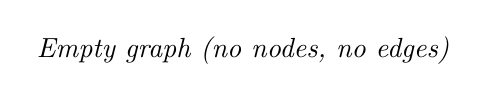
\begin{tikzpicture}
        \node at (0,0) {\textit{Empty graph (no nodes, no edges)}};
    \end{tikzpicture}
    \end{center}
    \textbf{Terminating:} YES \quad \textbf{Confluent:} YES \quad \textbf{Unique Normal Forms:} YES
    
    \paragraph{ARS 2: $A = \{a\}$, $R = \{\}$}
    \begin{center}
    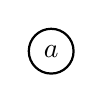
\begin{tikzpicture}[node distance=2cm, auto, thick]
        \node[circle, draw] (a) {$a$};
    \end{tikzpicture}
    \end{center}
    \textbf{Terminating:} YES \quad \textbf{Confluent:} YES \quad \textbf{Unique Normal Forms:} YES
    
    \paragraph{ARS 3: $A = \{a\}$, $R = \{(a,a)\}$}
    \begin{center}
    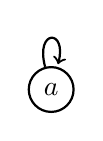
\begin{tikzpicture}[node distance=2cm, auto, thick, -latex]
        \node[circle, draw] (a) {$a$};
        \path (a) edge[loop above] (a);
    \end{tikzpicture}
    \end{center}
    \textbf{Terminating:} NO \quad \textbf{Confluent:} YES \quad \textbf{Unique Normal Forms:} NO
    
    \paragraph{ARS 4: $A = \{a,b,c\}$, $R = \{(a,b),(a,c)\}$}
    \begin{center}
    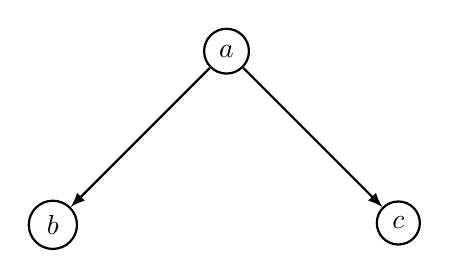
\begin{tikzpicture}[node distance=2.5cm, auto, thick, -latex]
        \node[circle, draw] (a) {$a$};
        \node[circle, draw] (b) [below left=of a] {$b$};
        \node[circle, draw] (c) [below right=of a] {$c$};
        
        \path (a) edge (b);
        \path (a) edge (c);
    \end{tikzpicture}
    \end{center}
    \textbf{Terminating:} YES \quad \textbf{Confluent:} NO \quad \textbf{Unique Normal Forms:} NO
    
    \paragraph{ARS 5: $A = \{a,b\}$, $R = \{(a,a),(a,b)\}$}
    \begin{center}
    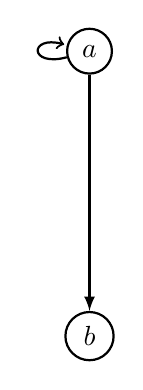
\begin{tikzpicture}[node distance=3cm, auto, thick, -latex]
        \node[circle, draw] (a) {$a$};
        \node[circle, draw] (b) [below=of a] {$b$};
        
        \path (a) edge[loop left] (a);
        \path (a) edge (b);
    \end{tikzpicture}
    \end{center}
    \textbf{Terminating:} NO \quad \textbf{Confluent:} NO \quad \textbf{Unique Normal Forms:} NO
    
    \paragraph{ARS 6: $A = \{a,b,c\}$, $R = \{(a,b),(b,b),(a,c)\}$}
    \begin{center}
    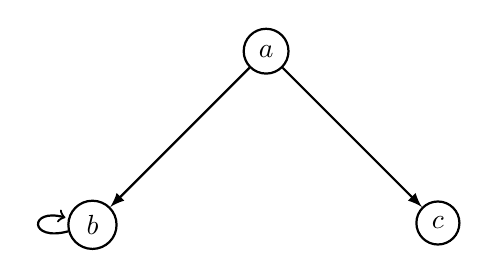
\begin{tikzpicture}[node distance=2.5cm, auto, thick, -latex]
        \node[circle, draw] (a) {$a$};
        \node[circle, draw] (b) [below left=of a] {$b$};
        \node[circle, draw] (c) [below right=of a] {$c$};
        
        \path (a) edge (b);
        \path (a) edge (c);
        \path (b) edge[loop left] (b);
    \end{tikzpicture}
    \end{center}
    \textbf{Terminating:} NO \quad \textbf{Confluent:} NO \quad \textbf{Unique Normal Forms:} NO
    
    \paragraph{ARS 7: $A = \{a,b,c\}$, $R = \{(a,b),(b,b),(a,c),(c,c)\}$}
    \begin{center}
    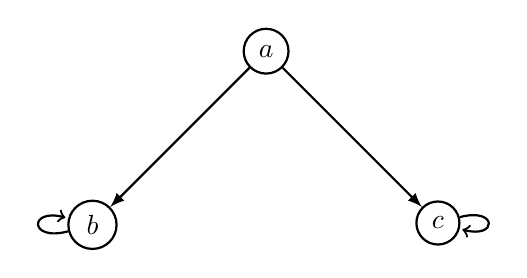
\begin{tikzpicture}[node distance=2.5cm, auto, thick, -latex]
        \node[circle, draw] (a) {$a$};
        \node[circle, draw] (b) [below left=of a] {$b$};
        \node[circle, draw] (c) [below right=of a] {$c$};
        
        \path (a) edge (b);
        \path (a) edge (c);
        \path (b) edge[loop left] (b);
        \path (c) edge[loop right] (c);
    \end{tikzpicture}
    \end{center}
    \textbf{Terminating:} NO \quad \textbf{Confluent:} NO \quad \textbf{Unique Normal Forms:} NO

    \paragraph{8 Combinations Table}
    \begin{center}
        \begin{tabular}{|c|c|c|l|}
        \hline
        \textbf{Confluent} & \textbf{Terminating} & \textbf{Unique NF} & \textbf{Example} \\
        \hline
        True & True & True & $A = \{a\}$, $R = \{\}$ \\
        True & True & False & $A = \{\}$, $R = \{\}$ \\
        True & False & True & $A = \{a,b\}$, $R = \{(a,b),(b,b)\}$ \\
        True & False & False & $A = \{a\}$, $R = \{(a,a)\}$ \\
        False & True & True & $A = \{a,b,c,d\}$, $R = \{(a,b),(a,c),(c,d)\}$ \\
        False & True & False & $A = \{a,b,c\}$, $R = \{(a,b),(a,c)\}$ \\
        False & False & True & $A = \{a,b,c\}$, $R = \{(a,b),(b,a),(a,c),(c,a)\}$ \\
        False & False & False & $A = \{a,b,c\}$, $R = \{(a,b),(b,b),(a,c)\}$ \\
        \hline
        \end{tabular}
    \end{center}

    \paragraph{Examples for 8 Combinations}

    \subparagraph{Example 1: Confluent=T, Terminating=T, Unique Normal Forms=T}
    $A = \{a\}$, $R = \{\}$
    \begin{center}
    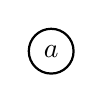
\begin{tikzpicture}[node distance=2cm, auto, thick]
        \node[circle, draw] (a) {$a$};
    \end{tikzpicture}
    \end{center}

    \subparagraph{Example 2: Confluent=T, Terminating=T, Unique Normal Forms=F}
    $A = \{\}$, $R = \{\}$
    \begin{center}
    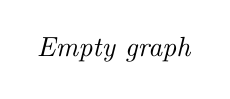
\begin{tikzpicture}
        \node at (0,0) {\textit{Empty graph}};
    \end{tikzpicture}
    \end{center}

    \subparagraph{Example 3: Confluent=T, Terminating=F, Unique Normal Forms=T}
    $A = \{a,b\}$, $R = \{(a,b),(b,b)\}$
    \begin{center}
    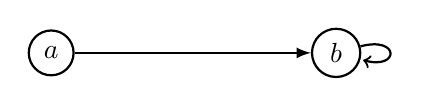
\begin{tikzpicture}[node distance=3cm, auto, thick, -latex]
        \node[circle, draw] (a) {$a$};
        \node[circle, draw] (b) [right=of a] {$b$};
        
        \path (a) edge (b);
        \path (b) edge[loop right] (b);
    \end{tikzpicture}
    \end{center}

    \subparagraph{Example 4: Confluent=T, Terminating=F, Unique Normal Forms=F}
    $A = \{a\}$, $R = \{(a,a)\}$
    \begin{center}
    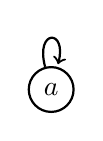
\begin{tikzpicture}[node distance=2cm, auto, thick, -latex]
        \node[circle, draw] (a) {$a$};
        \path (a) edge[loop above] (a);
    \end{tikzpicture}
    \end{center}

    \subparagraph{Example 5: Confluent=F, Terminating=T, Unique Normal Forms=T}
    $A = \{a,b,c,d\}$, $R = \{(a,b),(a,c),(c,d)\}$
    \begin{center}
        \begin{tikzpicture}[node distance=2.5cm, auto, thick, -latex]
            \node[circle, draw] (a) {$a$};
            \node[circle, draw] (b) [below left=of a] {$b$};
            \node[circle, draw] (c) [below right=of a] {$c$};
            \node[circle, draw] (d) [below=of c] {$d$};
            
            \path (a) edge (b);
            \path (a) edge (c);
            \path (c) edge (d);
        \end{tikzpicture}
    \end{center}

    \subparagraph{Example 6: Confluent=F, Terminating=T, Unique Normal Forms=F}
    $A = \{a,b,c\}$, $R = \{(a,b),(a,c)\}$
    \begin{center}
        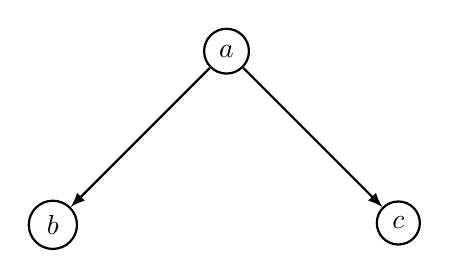
\begin{tikzpicture}[node distance=2.5cm, auto, thick, -latex]
            \node[circle, draw] (a) {$a$};
            \node[circle, draw] (b) [below left=of a] {$b$};
            \node[circle, draw] (c) [below right=of a] {$c$};
            
            \path (a) edge (b);
            \path (a) edge (c);
        \end{tikzpicture}
    \end{center}

    \subparagraph{Example 7: Confluent=F, Terminating=F, Unique Normal Forms=T}
    $A = \{a,b,c\}$, $R = \{(a,b),(b,a),(a,c),(c,a)\}$
    \begin{center}
    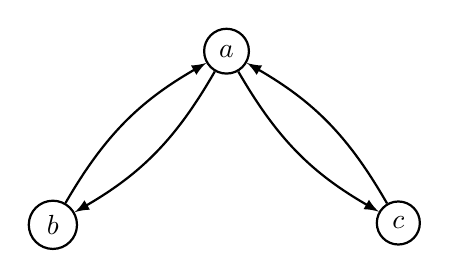
\begin{tikzpicture}[node distance=2.5cm, auto, thick, -latex]
        \node[circle, draw] (a) {$a$};
        \node[circle, draw] (b) [below left=of a] {$b$};
        \node[circle, draw] (c) [below right=of a] {$c$};
        
        \path (a) edge[bend left=15] (b);
        \path (b) edge[bend left=15] (a);
        \path (a) edge[bend right=15] (c);
        \path (c) edge[bend right=15] (a);
    \end{tikzpicture}
    \end{center}

    \subparagraph{Example 8: Confluent=F, Terminating=F, Unique Normal Forms=F}
    $A = \{a,b,c\}$, $R = \{(a,b),(b,b),(a,c)\}$
    \begin{center}
    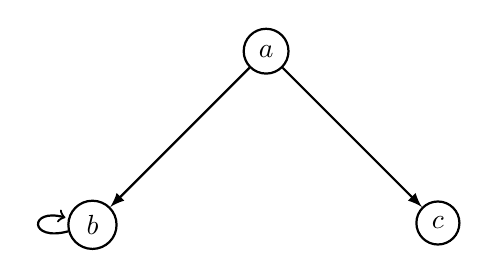
\begin{tikzpicture}[node distance=2.5cm, auto, thick, -latex]
        \node[circle, draw] (a) {$a$};
        \node[circle, draw] (b) [below left=of a] {$b$};
        \node[circle, draw] (c) [below right=of a] {$c$};
        
        \path (a) edge (b);
        \path (a) edge (c);
        \path (b) edge[loop left] (b);
    \end{tikzpicture}
    \end{center}

    \subsubsection{Exploration}
    Abstract Reduction Systems provide a mathematical foundation for understanding computation and rewriting. The properties of termination, confluence, and unique normal forms are fundamental to understanding how programming languages behave:
    
    \begin{itemize}
    \item \textbf{Termination} ensures that computations eventually halt
    \item \textbf{Confluence} guarantees that the order of operations doesn't affect the final result
    \item \textbf{Unique Normal Forms} means every expression has a single, well-defined simplified form
    \end{itemize}
    
    These concepts directly apply to programming language design, where we want predictable evaluation strategies and guaranteed termination for certain classes of programs.
    
    \subsubsection{Questions}
    1. How do the termination properties of ARSs relate to the halting problem in computation?\newline
    2. Why might a programming language designer prefer confluent systems over non-confluent ones?\newline

\subsection{Week 3}
\subsubsection{Homework}
\subsubsection{Exploration}
\subsubsection{Questions}

\subsection{Week 4}
\subsubsection{Homework}
\subsubsection{Exploration}
\subsubsection{Questions}

\subsection{Week 5}
\subsubsection{Homework}
\subsubsection{Exploration}
\subsubsection{Questions}

\subsection{Week 6}
\subsubsection{Homework}
\subsubsection{Exploration}
\subsubsection{Questions}

\subsection{Week 7}
\subsubsection{Homework}
\subsubsection{Exploration}
\subsubsection{Questions}

\subsection{Week 8}
\subsubsection{Homework}
\subsubsection{Exploration}
\subsubsection{Questions}

\subsection{Week 9}
\subsubsection{Homework}
\subsubsection{Exploration}
\subsubsection{Questions}

\subsection{Week 10}
\subsubsection{Homework}
\subsubsection{Exploration}
\subsubsection{Questions}

\subsection{Week 11}
\subsubsection{Homework}
\subsubsection{Exploration}
\subsubsection{Questions}

\section{Synthesis}

\section{Evidence of Participation}

\section{Conclusion}\label{conclusion}

\begin{thebibliography}{9}
\end{thebibliography}

\end{document}
